\documentclass{standalone}

\usepackage[T1]{fontenc}
\usepackage{amsmath,amssymb,mathtools}
\newcommand{\set}[1]{\left\{ #1 \right \}}

\usepackage{graphicx}
\definecolor{navyblue}{RGB}{0,0,128}
\begin{document}
\begin{tikzpicture}
    
    \node[] (1) {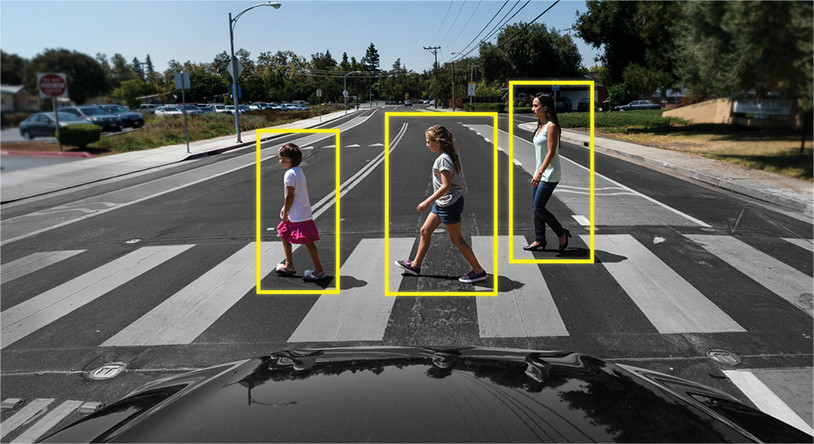
\includegraphics[width=0.45\textwidth]{pedestrian.jpg}};
    \node[below of = 1, draw=green, fill=green!10!white, rectangle, inner
    sep=0.2cm, minimum width=4.85cm] (2) {Pedestrian};
    \node[right of=1, xshift=2.25cm] (3) {{\Huge +}};
    \node[right of=3, xshift=1cm] (4) {
\includegraphics[width=0.25\textwidth]{noise.png}};
    \node[right of=4, xshift=1cm] (5) {{\Huge =}};
    \node[right of=5, xshift=2.2cm] (6) {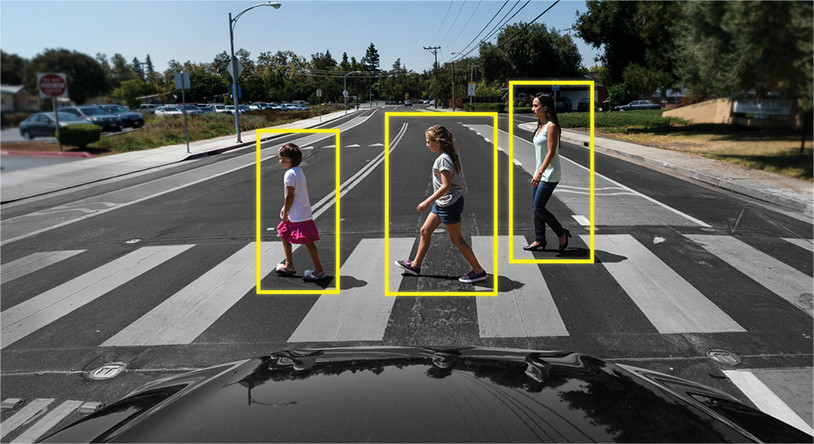
\includegraphics[width=0.45\textwidth]{pedestrian.jpg}};

    \node[below of = 6, draw=red, fill=red!10!white, rectangle, inner
    sep=0.2cm, minimum width=4.85cm] (2) {NOT Pedestrian};
    \end{tikzpicture}
\end{document}
